\documentclass{book}

\usepackage{amssymb}
\usepackage{amsmath}
\usepackage{amsthm}
\usepackage{arydshln}
\usepackage{calc}
\usepackage{cancel}
\usepackage{caption}
\usepackage{cite}
\usepackage{color}
\usepackage{enumitem}
\usepackage{esint}
\usepackage{etoolbox}
\usepackage{float}
\usepackage{framed}
\usepackage{fullpage}
\usepackage{gensymb}
\usepackage[margin=1in]{geometry}
\usepackage{graphicx}
\usepackage{listings}
\usepackage{multirow}
\usepackage{subfiles}
\usepackage{rsfso}
\usepackage{tikz}
\usepackage{tikz-3dplot}
\usepackage{ushort}
\usepackage{wrapfig}
\usepackage{xcolor}
\usepackage{soul}
\usepackage{epstopdf}

% pdf versions
\pdfoptionpdfminorversion=7

% handle page stretching
\raggedbottom

% Graphics file location
\graphicspath{{Graphics/}{../Graphics/}}

% Use for drawings
\usetikzlibrary{angles,arrows,calc,decorations,intersections,patterns,positioning,quotes}
\newcommand{\midarrow}{\tikz \draw[-latex] (0,0) -- +(.1,0);}

% Tikz commands for drawing block diagrams, etc...
\tikzset{%
	block/.style    = {draw, rectangle, minimum height = 2em, minimum width = 2em},
	sum/.style      = {draw, circle}, % Adder
	input/.style    = {fill=white, rectangle}, % Input
	output/.style   = {fill=white, rectangle}, % Output
	waypoint/.style   = {coordinate}, % Output
}

\tikzset{
	saveuse path/.code 2 args={
		\pgfkeysalso{#1/.style={insert path={#2}}}%
		\global\expandafter\let\csname pgfk@\pgfkeyscurrentpath/.@cmd\expandafter\endcsname
		% not optimal as it is now global through out the document
		\csname pgfk@\pgfkeyscurrentpath/.@cmd\endcsname
		\pgfkeysalso{#1}},
	/pgf/math set seed/.code=\pgfmathsetseed{#1}}

% Define Laplace, Fourier transform symbols
\newcommand{\LT}{\mathcal{L}}
\newcommand{\FT}{\mathcal{F}}

% Define adjugate function
\newcommand{\adj}{\text{adj}}

% Define rank function
\newcommand{\rank}{\text{rank}}

% commands to speed up writing j\omega and s-plane
\newcommand{\jw}{j\omega}
\newcommand{\spl}{s\textrm{-plane}}
% Clean up overline/underline for math mode
\def\obar#1{\bar{#1}}
\def\ubar#1{\ushort{#1}}

\newcommand{\exmp}{\subsubsection*{Example}}
\newcommand{\nib}{\noindent$ \bullet\ $}


\begin{document}
	\chapter*{Lecture 10}
	\section*{Control System Design Methods}
	\begin{center}
		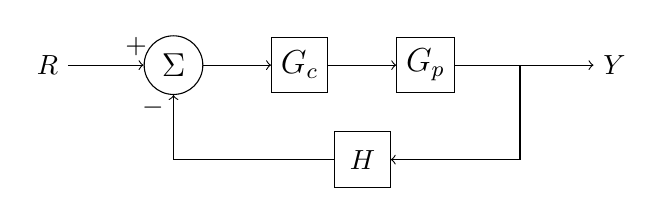
\begin{tikzpicture}[node distance = 1.6cm]
		\node[input] (r) at (0,0) {$ R $};
		\node[sum,right of=r] (sum) {\large$ \Sigma $};
		\node[block, right of=sum] (gc) {\large$ G_c $};
		\node[block, right of=gc] (gp) {\large$ G_p $};
		\node[block] (H) at (4,-1.2) {$ H $};
		\node[output, right of=gp, node distance = 2.4cm] (y) {$ Y $};
		\draw[->] (r) -- node[above,pos=0.9] {$ + $} (sum);
		\draw[->] (sum) -- (gc);
		\draw[->] (gc) -- (gp);
		\draw[->] (gp) -- (y);
		\draw[->] ($(gp)!0.5!(y)$) |- (H);
		\draw[->] (H) -| node[left,pos=0.9] {$ - $} (sum);
		\end{tikzpicture}
	\end{center}
	This figure shows a typical control system. The plant $ G_p $ is known, and we are to come up with $ G_c $ such that $ y(t) \approx r(t)$ to within given specifications. $ H(s) $ is the sensor transfer function and is considered known. So, our job is to design $ G_c $ to meet the given specs.\\
	
	%	\noindent Some common controller types are
	%	\begin{itemize}
	%		\item Proportional --- $ G_c=K_p $
	%		\item Proportional-Integral (PI) --- $ G_c=K_p + K_i\frac{1}{s} $
	%		\item Proportaional-Derivative (PD) --- $ G_c=K_p + K_ds $
	%		\item Proportional-Integral-Derivative (PID) --- $ G_c=K_p + K_i\frac{1}{s} + K_ds  $
	%		\item Lead --- $ G_c=K_c\dfrac{\frac{s}{\omega_1}+1}{\frac{s}{\omega_2}+1} $, $ \omega_1 < \omega_2 $
	%		\item Lag --- $ G_c=K_c\dfrac{\frac{s}{\omega_1}+1}{\frac{s}{\omega_2}+1} $, $ \omega_1 > \omega_2 $
	%		\item Lead-lag or Lag-lead --- $ G_c=K_c\dfrac{\frac{s}{\omega_1}+1}{\frac{s}{\omega_2}+1}\dfrac{\frac{s}{\omega_3}+1}{\frac{s}{\omega_4}+1} $
	%	\end{itemize}
	There are several different ways to do the job:
	\begin{itemize}
		\item Frequency response methods:
		\begin{itemize}
			\item Analytical methods (loop shaping)
			\item Graphical methods (root locus design)
		\end{itemize}
		\item State-space design methods
	\end{itemize}
	We will start by discussion Root Locus design. 
	
	\section*{Root Locus Design Methods}
	Root locus design is a graphical technique based on a system's ``Root Locus''. This method was developed in 1948 by Walter R. Evans, an aircraft engineer.
	
	Let's discuss the \textbf{root locus}: The root locus of a feedback system is a diagram which shows how the system's closed-loop poles migrate in the complex plane ($ s- $plane) as some parameter of the system is varied.
	
	\exmp
	Consider the feedback system shown below:
	\begin{center}
		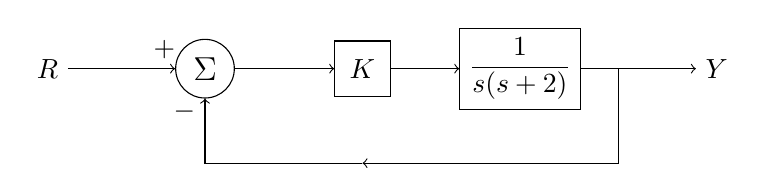
\begin{tikzpicture}[node distance = 2cm]
		\node[input] (r) at (0,0) {$ R $};
		\node[sum,right of=r] (sum) {\large$ \Sigma $};
		\node[block, right of=sum] (gc) {$ K $};
		\node[block, right of=gc] (gp) {$ \dfrac{1}{s(s+2)} $};
		\node[waypoint] (H) at (4,-1.2) {$ H $};
		\node[output, right of=gp, node distance = 2.5cm] (y) {$ Y $};
		\draw[->] (r) -- node[above,pos=0.9] {$ + $} (sum);
		\draw[->] (sum) -- (gc);
		\draw[->] (gc) -- (gp);
		\draw[->] (gp) -- (y);
		\draw[->] ($(gp)!0.5!(y)$) |- (H);
		\draw[->] (H) -| node[left,pos=0.9] {$ - $} (sum);
		\end{tikzpicture}
	\end{center}
	We wish to ``see'' how the parameter $ K $ affects the location of the closed-loop poles of the above system.
	\begin{enumerate}
		\item Determine the closed-loop transfer function:
		\[ \frac{Y}{R}(s) = \frac{\dfrac{K}{s(s+2)}}{1+\dfrac{K}{s(s+2)}} = \dfrac{K}{s^2+2s+K} \]
		\item Determine the pole locations: Solve the characteristic equation.
		\[ s^2+2s+K = 0  \quad\Longrightarrow\quad s = -1\pm\sqrt{1-K} \]
		So, $ s_1 = -1+\sqrt{1-K} $ and $ s_2 = -1-\sqrt{1-K} $. Then,
		\[ 	\begin{array}{c |c| c}
		K & s_1 & s_2 \\ \hline
		0 & 0 & -2  \\
		3/4 & -1/2  & -3/2  \\
		1 & -1 & -1 \\
		2 & -1+j & -1-j \\
		3 & -1+j\sqrt{2} & -1-j\sqrt{2}\\
		\end{array} \]
		\[ \text{etc...} \]
		\begin{center}
			\begin{tikzpicture}[xscale=2,yscale=1.25]
			\draw[<->] (-3,0) -- (1.5,0) node[below left] {Re};
			\draw[<->] (0,-1.5) -- (0,1.5) node[below left] {Im};
			\draw[thick] (-2,0.01) node {\Large$ \times $} -- (-0,0.01) node {\Large$ \times $};
			\draw[thick,latex-latex] (-1,-2) -- (-1,2);
			\node at (-1.5,0) {$ \bullet $};
			\node at (-0.5,0) {$ \bullet $};
			\node at (-1,0) {$ \bullet $};
			\node at (-1,1) {$ \bullet $};
			\node at (-1,1.414) {$ \bullet $};
			\node at (-1,-1) {$ \bullet $};
			\node at (-1,-1.414) {$ \bullet $};
			\node[above] at (-1.5,0) {$ K=3/4 $};
			\node[above] at (-0.5,0) {$ K=3/4 $};
			\node[below left] at (-1,0) {$ K=1 $};
			\node[left] at (-1,1) {$ K=2 $};
			\node[left] at (-1,-1) {$ K=2 $};
			\node[left] at (-1,1.414) {$ K=3 $};
			\node[left] at (-1,-1.414) {$ K=3 $};
			\end{tikzpicture}
		\end{center}
		
	\end{enumerate}
	
	The root locus shows the sets of points in the $ \spl $ occupied by the closed-loop poles of a control system as some parameter $ K $ is varied. How can this be of use to us?
	\begin{itemize}
		\item We know that the location of the closed-loop poles in the $ \spl $ translates to into transient response characteristics for a step input (at least in the case of a 2nd order system with no zeros).
		\item This means we can influence the performance of the system by picking a value of $ K $ that places the closed-loop poles at points that represent ``good'' $ \zeta $ and $ \omega_n $. 
	\end{itemize}
	
	For example, imagine a system where the step response is:
	\begin{itemize}
		\item $ y(t) $ is overdamped for $ 0 < K < 1 $
		\item $ y(t) $ is critically damped for $ K=1 $
		\item $ y(t) $ is underdamped for $ K>1 $
	\end{itemize}
	As K increases (above 1), $ \zeta $ decreases, thereby increasing overshoot. The root locus plot will let us easily relate the gain $ K $ to the damping $ \zeta $.
	
	\section*{Constructing the Root Locus}
	How can we construct root loci easily? We will now develop a set of rules for constructing the root locus of a system. Recall, root locus tells use how the closed-loop poles of a system migrate on the $ \spl $. Recall that we have a closed-loop transfer function
	\[ \frac{KL(s)}{1+KL(s)} \] 
	So, the location of closed-loop poles are given by the equation
	\begin{equation}
	1+KL(s) = 0 \quad\textrm{(C.L. characteristic eqn)}
	\end{equation}
	or in pole-zero form:
	\begin{equation}
	1+\frac{K(s+z_1)(s+z_2)\ldots(s+z_m)}{(s+p_1)(s+p_2)\ldots(s+p_n)} = 0
	\end{equation}
	where $ -z_i $ and $ -p_i $ are the zeros and poles of $ L(s) $, respectively. Also note that $ m\leq n $. 	We can rewrite (2) as
	\begin{equation}
	\frac{(s+z_1)(s+z_2)\ldots(s+z_m)}{(s+p_1)(s+p_2)\ldots(s+p_n)} = -\frac{1}{K}
	\end{equation}
	Any point $ s $ of the $ \spl $ (or complex plane) that satisfies this equation for some value of $ K $ is a point on the root locus.
	
	Let's say we are interested in the root locus for $ 0\leq K < \infty $. We observe that root loci always start ($ K=0 $) at the poles of $ L(s) $ and end ($ K\to\infty $) at the zeros of $ L(s) $ or at infinity (for $ m<n $). \textbf{This is the first rule for drawing root loci}. In other words, to construct the root locus of a closed-loop system, start by constructing the pole-zero plot of $ L(s) $. Root locus branches will start from poles of $ L(s) $ and end at zeros of $ L(s) $ or infinity.
	
	The next two root-locus rules are easily inferred from equation (3):
	
	\paragraph*{Rule 2:} There are $ n $ branches (as many branches are the number of poles of $ L(s) $).
	\paragraph*{Rule 3:} Root locus branches are symmetric about the real axis. This comes from the fact that $ 1+L(s)=0 $ are the roots of a real polynomial, and the roots of a real polynomial will either be all real, or if their are any complex roots, they must appear as a complex conjugate pair.
	
	\vspace{1em}
	
	\begin{center}
		\begin{tikzpicture}[xscale=2,yscale=1.25]
		\draw[<->] (-4,0) -- (1,0) node[below left] {Re};
		\draw[<->] (0,-1.5) -- (0,1.5) node[below left] {Im};
		\draw[thick] (-1,0.01) node {\Large$ \times $} -- (-0,0.01) node {\Large$ \times $};
		\draw[thick] (-2,0.01) node {\Large$ \circ $} -- (-3,0.01) node {\Large$ \circ $};
		\draw[thick,latex-latex] (-1.5,-1) arc (-90:90:1);
		\draw[thick] (-1.5,-1) arc (270:90:1);
		\end{tikzpicture}\\
		Possible
		
		\vspace{2em}
		
		\begin{tikzpicture}[xscale=2,yscale=1.25]
		\draw[<->] (-4,0) -- (1,0) node[below left] {Re};
		\draw[<->] (0,-1.5) -- (0,1.5) node[below left] {Im};
		\node at (-1,0.01)  {\Large$ \times $};
		\node at (-0,0.01)  {\Large$ \times $};
		\node at (-2,0.01)  {\Large$ \circ $};
		\node at (-3,0.01)  {\Large$ \circ $};
		\draw[thick,-latex] (-1,0) arc (0:90:0.5 and 0.75);
		\draw[thick] (-2,0) arc (180:90:0.5 and 0.75);
		\draw[thick,-latex] (0,0) arc (0:-90:1.5 and 1);
		\draw[thick] (-3,0) arc (-180:-90:1.5 and 1);
		\end{tikzpicture}\\
		Not Possible
	\end{center}
	
	\noindent\textbf{Note: In the above diagrams, the root loci should all follow circular paths when off the real axis; they are drawn as ellipses for the sake of saving space.}
	
	\section*{Complex Number Review}
	To understand how the next few rules come about, we need to first review complex numbers and their representation. Any complex number can be written as:
	\begin{equation}
	s = \sigma + \jw
	\end{equation}
	where $ \sigma $ is the real part of $ s $ and $ \omega $ is the imaginary part of $ s $.
	
	$ s $ can be represented in the $ \spl $ in a couple of ways:
	\begin{itemize}
		\item as a point in the complex plane with ``coordinates'' $ (\sigma,\omega) $.
		\item or, view $ s $ as a vector in the complex plane with the tail at the origin and the tip at the point $ P $ with coordinates $ (\sigma,\omega) $. Then, the magnitude of the vector is $ M $ (called the modulus of $ s $) and the angle the vector makes with the positive real axis is $ \theta $ (called the argument of $ s $).
	\end{itemize}
	
	\begin{center}
		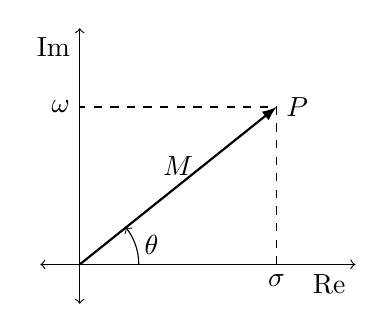
\begin{tikzpicture}
		\draw[<->]  (-0.5,0) -- (3.5,0);  % x Axis
		\draw[<->]  (0,-0.5) -- (0,3);  % y Axis
		\node[below left] at (3.5,0) {Re};
		\node[below left] at (0,3) {Im};
		
		\node[right] at (2.5,2) {$ P $};
		
		\draw[thick,-latex] (0,0) -- (2.5,2);
		
		\node[above] at (1.25,1) {$ M $};
		
		\draw[->] (0.75,0) arc (0:39:0.75);
		\node[right] at (0.7,0.25) {$ \theta $};
		
		\draw[dashed] (2.5,0) -- (2.5,2) -- (0,2);
		\node[below] at (2.5,0) {$ \sigma $};
		\node[left] at (0,2) {$ \omega $};
		\end{tikzpicture}
	\end{center}
	
	Using $ M $ and $ \theta $, we can write
	\begin{equation}
	s = Me^{j\theta}
	\end{equation}
	called the polar representation of $ s $.
	
	Why are (4) and (5) equivalent? We know that
	\[
	e^{j\theta}=\cos\theta+j\sin\theta \quad\textrm{(Euler's Theorem)}
	\]
	
	\subsection*{Proof}
	Recall the Taylor series expansion of $ e^x $:
	\[ e^x = 1+ x+ \frac{x^2}{2!}+\frac{x^3}{3!}+\ldots \]
	Then,
	\[ e^{j\theta} = 1+ {j\theta}+ \frac{({j\theta})^2}{2!}+\frac{({j\theta})^3}{3!}+\ldots \]
	where $ j=\sqrt{-1} $.
	
	Collecting the real and complex terms together, we have:
	\[ e^{j\theta} = \underbrace{1-\frac{\theta^2}{2!}+\frac{\theta^4}{4!}-\ldots}_{\cos\theta} + j\Big(\underbrace{\theta-\frac{\theta^3}{3!}+\frac{\theta^5}{5!}-\ldots}_{\sin\theta}\Big) \]
	So,
	\[
	e^{j\theta}=\cos\theta+j\sin\theta \quad\textrm{(Euler's Theorem)}
	\]
	Similarly,
	\[e^{-j\theta}=\cos\theta-j\sin\theta\]
	\[ \cos\theta=\frac{1}{2}\left(e^{j\theta}+e^{-j\theta}\right) \]
	\[ \sin\theta=\frac{1}{2j}\left(e^{j\theta}-e^{-j\theta}\right) \]
	\textbf{(end proof)}
	
	So, from (5):
	\begin{equation}
	Me^{j\theta} = M\cos\theta+jM\sin\theta
	\end{equation}
	which is true to the figure shown.
	
	So, we have
	\[ s = \sigma + \jw = Me^{j\theta} \]
	where
	\[ M=\sqrt{\sigma^2+\omega^2}\quad\textrm{and}\quad\theta=\tan^{-1}\left(\frac{\omega}{\sigma}\right) \]
	
	The useful thing about the polar representation is that it's easy to deal with products and ratios of complex numbers.
	
	Example:
	\[ s_1 = \sigma_1 + \jw_1 = M_1e^{j\theta_1} \]
	\[ s_2 = \sigma_2 + \jw_2 = M_2e^{j\theta_2} \]
	\[ s_1s_2 = (\sigma_1 + \jw_1)(\sigma_2 + \jw_2) = M_1e^{j\theta_1}\cdot M_2e^{j\theta_2} = M_1M_2e^{j(\theta_1+\theta_2)} \]
	$ \Longrightarrow $ The modulus of a product equals the product of the moduli.
	$ \Longrightarrow $ The argument of a product equals the sum of arguments.
	
	Similarly, we find:
	\[ \frac{s_1}{s_2} = \frac{M_1}{M_2}e^{j(\theta_1-\theta_2)} \]
	$ \Longrightarrow $ The modulus of a ratio equals the ratio of the moduli.
	$ \Longrightarrow $ The argument of a ratio equals the difference of arguments.
	
	\section*{Angle and Magnitude Criterion}
	Before moving on to Rule 4, let's look at how to graphically solve functions of complex variables.
	If $ s_1 = \sigma_1 + \jw_1 = M_1e^{j\theta_1} $, then 
	\[ s_1+a = (\sigma_1+a) + \jw_1 = M_1'e^{j\theta_1'} \]
	where $ a $ is  positive real number
	\begin{center}
		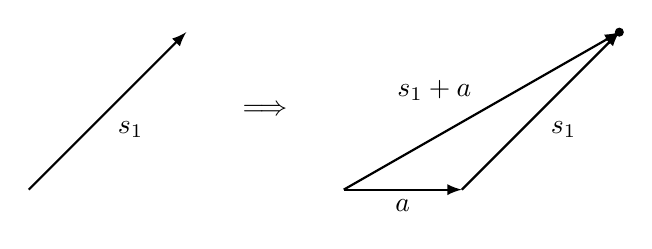
\begin{tikzpicture}
		\draw[thick,-latex] (-4,0) -- node[below right] {$ s_1 $} (-2,2);
		\node at (-1,1) {$ \Longrightarrow $};
		\draw[thick,-latex] (0,0) -- node[below] {$ a $} (1.5,0);
		\draw[thick,-latex] (1.5,0) -- node[below right] {$ s_1 $} (3.5,2);
		\draw[thick,-latex] (0,0) -- node[above left] {$ s_1+a $} (3.5,2);
		\draw[fill=black] (3.5,2) circle (0.05);
		\end{tikzpicture}
	\end{center}
	Now, consider a function $ F(s) = s+a $ and evaluate $ F(s) $ at $ s=s_1 $. To do this graphically:
	\begin{enumerate}
		
		\item locate the point $ s_1 $,
		\item locate the zero of $ F(s) $,
		\item draw the vector from the zero of $ F(s) $ to the point $ s_1 $.
	\end{enumerate}
	\begin{center}
		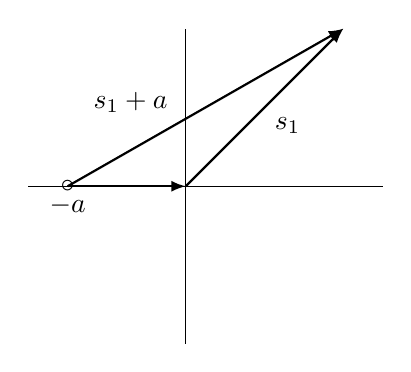
\begin{tikzpicture}
		\node at (0,0) {$ \circ $};
		\node[below] at (0,0) {$ -a $};
		\draw[thick,-latex] (0,0) -- (1.5,0);
		\draw[thick,-latex] (1.5,0) -- node[below right] {$ s_1 $} (3.5,2);
		\draw[thick,-latex] (0,0) -- node[above left,pos=0.4] {$ s_1+a $} (3.5,2);
		\draw (1.5,-2) -- (1.5,2);
		\draw (-0.5,0) -- (4,0);
		\end{tikzpicture}
	\end{center}
	The solution to $ F(s)\big|_{s=s_1} $ is a vector drawn from the zero of $ F(s) $ to $ s_1 $. We can convert that answer to polar or Cartesian form.
	
	\exmp
	Graphically evaluate $ F(s)=s+4 $ for $ s=1+5i $.
	\begin{center}
		\begin{tikzpicture}[scale = 0.5]
		\draw (-6,0) -- (2,0);
		\draw (0,-2) -- (0,6);
		\node at (-4,0) {$ \circ $};
		\node[below] at (-4,0) {$ -4 $};
		\foreach \x in {-4,-3,-2,-1,0,1}
		\draw (\x cm,2pt) -- (\x cm,-2pt);
		\foreach \y in {0,1,2,3,4,5}
		\draw (2pt,\y cm) -- (-2pt,\y cm);
		\draw[thick,-latex] (-4,0) -- node[above left,pos=0.4] {$ M $} (1,5) node[above right] {$ 1+5i $};
		\draw (-2,0) arc (0:45:2);
		\node[right] at (-2,1) {$ \theta $};
		\end{tikzpicture}
	\end{center}
	What is the polar form equivalent?
	\[ F(s)\big|_{s=1+5i}=Me^{i\theta}=\sqrt{50}e^{i\frac{\pi}{4}} \]
	
	\exmp
	Graphically evaluate $ F(s)=\frac{s+1}{(s-1)(s+5)} $ for $ s=1+5i $.
	\[ F(s)\big|_{s=1+5i}=\frac{(s+1)\big|_{s=1+5i}}{(s-1)\big|_{s=1+5i}(s+5)\big|_{s=1+5i}} \]
	Consider each element independently:
	\begin{center}
		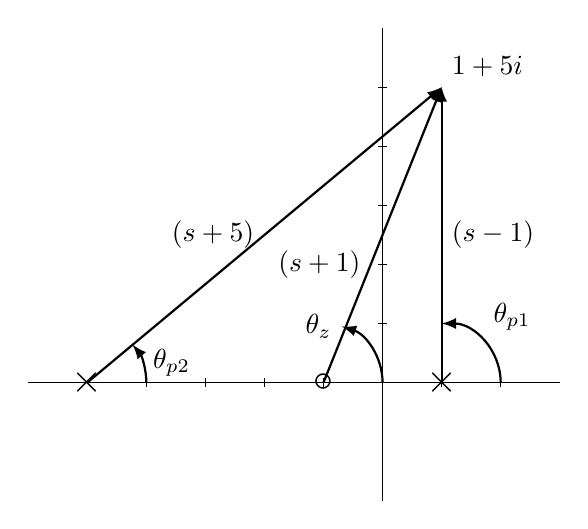
\begin{tikzpicture}[scale = 0.75]
		\draw (-6,0) -- (3,0);
		\draw (0,-2) -- (0,6);
		\foreach \x in {-4,-3,-2,-1,0,1,2}
		\draw (\x cm,2pt) -- (\x cm,-2pt);
		\foreach \y in {0,1,2,3,4,5}
		\draw (2pt,\y cm) -- (-2pt,\y cm);
		\node at (-1,0) {\Large$ \circ $};
		\draw[thick,-latex] (-1,0) -- node[left,pos=0.4] {$ (s+1) $} (1,5) node[above right] {$ 1+5i $};
		\node at (1,0) {\Large$ \times $};
		\draw[thick,-latex] (1,0) -- node[right] {$ (s-1) $} (1,5);
		\node at (-5,0) {\Large$ \times $};
		\draw[thick,-latex] (-5,0) -- node[left] {$ (s+5) $} (1,5);
		
		
		\draw[thick,-latex] (2,0) arc (0:90:1) node[above right,pos=0.5] {$ \theta_{p1} $};
		\draw[thick,-latex] (0,0) arc (0:72:1) node[left] {$ \theta_{z} $};
		\draw[thick,-latex] (-4,0) arc (0:40:1) node[right,pos=0.5] {$ \theta_{p2} $};
		\end{tikzpicture}
	\end{center}
	What is the polar form equivalent? Remember the rules for moduli and arguments for products and ratios.
	\[ F(s)\big|_{s=1+5i}=\frac{M_{z1}e^{j\theta_{z1}}}{(M_{p1}e^{j\theta_{p1}})(M_{p2}e^{j\theta_{p2}})} \]
	\[ F(s)\big|_{s=1+5i}=\frac{M_{z1}}{M_{p1}M_{p2}} e^{j(\theta_{z1}-\theta_{p1}-\theta_{p2})} \]
	
	In general, for $ F(s) = \frac{(s+z_1)(s+z_2)\ldots(s+z_m)}{(s+p_1)(s+p_2)\ldots(s+p_n)} $,
	\[ F(s) = \frac{M_{z1}M_{z2}\ldots M_{zm}}{M_{p1}M_{p2}\ldots M_{pn}} e^{j(\theta_{z1}+\theta_{z2}+\ldots+\theta_{zm}-\theta_{p1}-\theta_{p2}-\ldots-\theta_{pn})} \]
	Or,
	\begin{equation}
	F(s) = \frac{\prod^{m}M_{zi}}{\prod^{n}M_{pi}} e^{j\left(\sum^{m}\theta_{zi}-\sum^{n}\theta_{pi}\right)}
	\end{equation}
	\begin{itemize}
		\item[$ M $'s:] Length of vectors connecting poles/zeros to $ s $.
		\item[$ \theta $'s:] Angle of vectors connecting poles/zeros to $ s $.
	\end{itemize}
	
	Now, let's relate this to the root locus. As discussed previously, the root locus is the set of points where
	\[ L(s)=\frac{(s+z_1)(s+z_2)\ldots(s+z_m)}{(s+p_1)(s+p_2)\ldots(s+p_n)} = -\frac{1}{K}  \]
	
	What is the polar representation of $ -1/K $?
	\[ \frac{-1}{K} = \frac{1}{K}e^{j\cdot180^\circ} \]
	So,
	\begin{equation}
	\frac{\prod^{m}M_{zi}}{\prod^{n}M_{pi}} \nonumber e^{j\left(\sum^{m}\theta_{zi}-\sum^{n}\theta_{pi}\right)} = \frac{1}{K}e^{j\cdot180^\circ}
	\end{equation}
	By comparing the angle of the right and left side of this equation, we get the \textbf{Angle Criterion}:
	\begin{equation} \nonumber
	\sum^{m}\theta_{zi}-\sum^{n}\theta_{pi} = 180^\circ  \pm 360^\circ\ell = 180^\circ \cdot (1\pm 2\ell), \quad \ell = 0, 1, 2,\ldots
	\end{equation}
	(i.e., $\pm180^\circ \pm $ some multiple of $ 360^\circ $), by comparing the magnitude of the right and left side of this equation, we get the \textbf{Magnitude Criterion:}
	\begin{equation} \nonumber
	\frac{\prod^{n}M_{pi}}{\prod^{m}M_{zi}} = K
	\end{equation}
	\begin{center}
		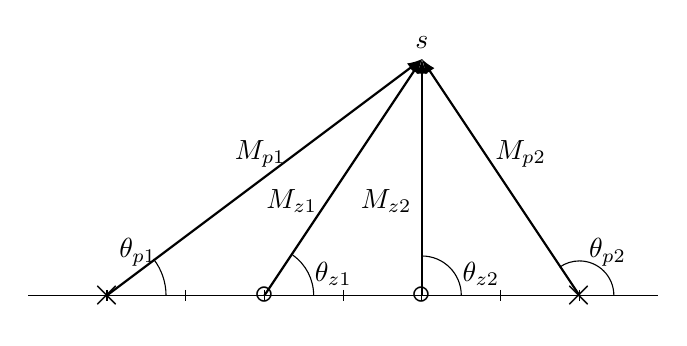
\begin{tikzpicture}[scale = 1]
		\draw (-7,0) -- (1,0);
		\foreach \x in {-6,-5,-4,-3,-2,-1,0}
		\draw (\x cm,2pt) -- (\x cm,-2pt);
		\node at (-6,0) {\Large$ \times $};
		\draw[thick,-latex] (-6,0) -- node[left,pos=0.6] {$ M_{p1} $} (-2,3) node[above] {$ s $};
		\draw (-5.25,0) arc (0:38:0.75);
		\node[above left] at (-5.25,0.25) {$ \theta_{p1} $};
		\node at (0,0) {\Large$ \times $};
		\draw[thick,-latex] (0,0) -- node[right,pos=0.6] {$ M_{p2} $} (-2,3);
		\draw (0.4375,0) arc (0:125:0.4375);
		\node[above right] at (0,0.25) {$ \theta_{p2} $};
		\node at (-4,0) {\Large$ \circ $};
		\draw[thick,-latex] (-4,0) -- node[left,pos=0.4] {$ M_{z1} $} (-2,3);
		\draw (-3.375,0) arc (0:55:0.625);
		\node[above] at (-3.125,0) {$ \theta_{z1} $};
		\node at (-2,0) {\Large$ \circ $};
		\draw[thick,-latex] (-2,0) -- node[left,pos=0.4] {$ M_{z2} $} (-2,3);
		\draw (-1.5,0) arc (0:90:0.5);
		\node[above] at (-1.25,0) {$ \theta_{z2} $};
		\end{tikzpicture}
	\end{center}
	\begin{itemize}
		\item If a point satisfies the Angle Criterion, then it is on the root locus.
		\item If and only if the point is on the root locus, the magnitude criterion gives us the $ K $ that will place a closed-loop pole there.
	\end{itemize}
	
	\exmp
	\begin{center}
		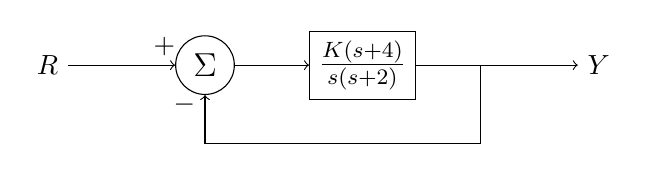
\begin{tikzpicture}[node distance = 2cm]
		\node[input] (r) at (0,0) {$ R $};
		\node[sum,right of=r] (sum) {\large$ \Sigma $};
		\node[block, right of=sum] (tf) {\large$ \frac{K(s+4)}{s(s+2)} $};
		\node[waypoint,below of=tf,node distance = 1cm] (wp) {};
		\node[output, right of=tf,node distance = 3cm] (y) {$ Y $};
		\draw[->] (r) -- node[above,pos=0.9] {$ + $} (sum);
		\draw[->] (sum) -- (tf);
		\draw[->] (tf) -- (y);
		\draw[->] ($(tf)!0.5!(y)$) |- (wp) -| node[left,pos=0.9] {$ - $} (sum);
		\end{tikzpicture}
	\end{center}
	Is $ s=-6+2j $ on the root locus? If so, what $ K $ will place a closed-loop pole there?
	\begin{center}
		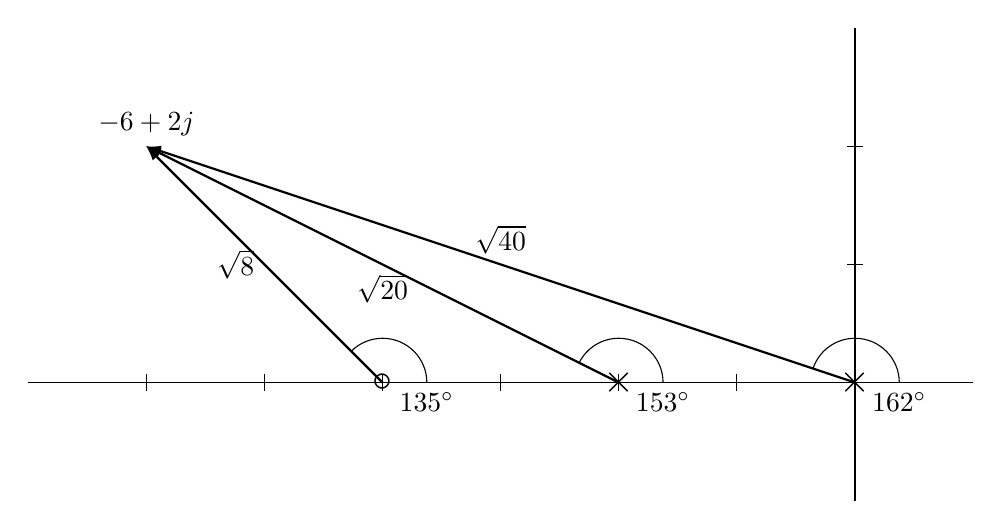
\begin{tikzpicture}[scale = 1.5]
		\draw (-7,0) -- (1,0);
		\foreach \x in {-6,-5,-4,-3,-2,-1,0}
		\draw (\x cm,2pt) -- (\x cm,-2pt);
		\draw (0,-1) -- (0,3);
		\foreach \x in {0,1,2}
		\draw (2pt,\x cm) -- (-2pt,\x cm);
		
		\node at (-4,0) {\Large$ \circ $};
		\draw[thick,-latex] (-4,0) -- node[left,pos=0.5] {$ \sqrt{8} $} (-6,2) node[above] {$ -6+2j $};
		\draw (-3.625,0) arc (0:135:0.375);
		\node[below] at (-3.625,0) {$ 135^\circ $};
		
		\node at (-2,0) {\Large$ \times $};
		\draw[thick,-latex] (-2,0) -- node[below,pos=0.5] {$ \sqrt{20} $} (-6,2);
		\draw (-1.625,0) arc (0:153:0.375);
		\node[below] at (-1.625,0) {$ 153^\circ $};
		
		\node at (0,0) {\Large$ \times $};
		\draw[thick,-latex] (0,0) -- node[above,pos=0.5] {$ \sqrt{40} $} (-6,2);
		\draw (0.375,0) arc (0:162:0.375);
		\node[below] at (0.375,0) {$ 162^\circ $};
		\end{tikzpicture}
	\end{center}
	Check angle criterion: Does $ \theta_z-\theta_{p1}-\theta_{p2} = 180 \pm \ell 360^\circ $?
	\[ 135^\circ-153^\circ-162^\circ=-180^\circ \quad \checkmark \]
	The point is on the root locus. Next we find the gain for this point:
	\[ K = \frac{M_{p1}M_{p2}}{M_z} = \frac{\sqrt{20}\sqrt{40}}{\sqrt{8}} = \sqrt{\frac{800}{8}} = 10 \]
	
	\section*{Real Axis of the Root Locus}
	Let's look at the real axis part of the root locus.
	\begin{center}
		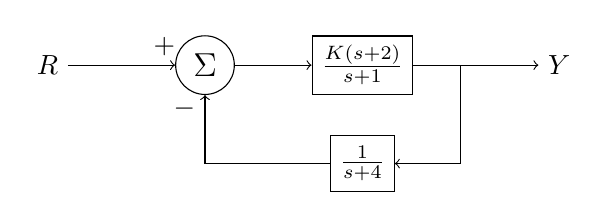
\begin{tikzpicture}[node distance = 2cm]
		\node[input] (r) at (0,0) {$ R $};
		\node[sum,right of=r] (sum) {\large$ \Sigma $};
		\node[block, right of=sum] (g) {$ \frac{K(s+2)}{s+1} $};
		\node[block,below of=g,node distance = 1.25cm] (h) {$ \frac{1}{s+4} $};
		\node[output, right of=g,node distance = 2.5cm] (y) {$ Y $};
		\draw[->] (r) -- node[above,pos=0.9] {$ + $} (sum);
		\draw[->] (sum) -- (g);
		\draw[->] (g) -- (y);
		\draw[->] ($(g)!0.5!(y)$) |- (h);
		\draw[->] (h) -| node[left,pos=0.9] {$ - $} (sum);
		
		\end{tikzpicture}
	\end{center}
	Open loop TF: $ \frac{K(s+2)}{(s+1)(s+4)} $.
	
	\begin{center}
		\begin{tikzpicture}[scale=0.75]
		\draw (-7,0) -- (2,0);
		\draw (0,-1.5) -- (0,1.5);
		\node at (-4,0) {\Large$ \times $};
		\node[below] at (-4,-0.05) {$ p_1 $};
		\draw[thick,-latex] (-4,0) -- (-7,0);
		\node at (-1,0) {\Large$ \times $};
		\node[below] at (-1,-0.05) {$ p_2 $};
		\draw[thick,-latex] (-1,0) -- (-2,0);
		\node at (-2,0) {\Large$ \circ $};
		\node[below] at (-2,-0.05) {$ z $};
		\end{tikzpicture}
	\end{center}
	Is $ s=0.5 $ on the root locus? Check the angle criterion:
	\[ \theta_z-\theta_{p1}-\theta_{p2} = 0 \neq 180^\circ\pm \ell360^\circ\]
	So, $ s=0.5 $ is not on the root locus. Are $ s=-1.5,\ -3,\ -5 $ on the root locus?
	\begin{align*}
	s=-1.5: &\quad 0-0-180 = -180 \qquad\quad \checkmark \textrm{on R.L.}\\
	s=-3:&\quad 180-0-180 = 0 \qquad\quad\ \times \textrm{not on R.L.}\\
	s=-5:&\quad 180-180-180 = -180 \quad \checkmark \textrm{on R.L.}
	\end{align*}
	
	What if we swap the locations of the $ p_1 $ pole and the zero $ z $?
	\begin{center}
		\begin{tikzpicture}[scale=0.75]
		\draw (-7,0) -- (2,0);
		\draw (0,-1.5) -- (0,1.5);
		\node at (-2,0) {\Large$ \times $};
		\node[below] at (-2,-0.05) {$ p_1 $};
		\draw[thick] (-4,0.01) -- (-7,0.01);
		\node at (-1,0) {\Large$ \times $};
		\node[below] at (-1,-0.05) {$ p_2 $};
		\draw[thick] (-1,0.01) -- (-2,0.01);
		\node at (-4,0) {\Large$ \circ $};
		\node[below] at (-4,-0.05) {$ z $};
		\end{tikzpicture}
	\end{center}
	\[ \theta_z-\theta_{p1}-\theta_{p2} = 0 \neq 180^\circ\pm \ell360^\circ\]
	\begin{align*}
	s=-0.5: &\quad 0-0-0 = 0 \qquad\quad \times \textrm{not on R.L.}\\
	s=-1.5: &\quad 0-0-180 = -180 \qquad\quad \checkmark \textrm{on R.L.}\\
	s=-3:&\quad 0-180-180 = -360 \qquad\quad\ \times \textrm{not on R.L.}\\
	s=-5:&\quad 180-180-180 = -180 \quad \checkmark \textrm{on R.L.}
	\end{align*}
	
	This leads to \textbf{Rule \#4} of root loci:
	\begin{itemize}
		\item[4.] The real axis part of the root locus lies to the left of an odd number of singularities (open loop poles/zeros) on the real axis.
	\end{itemize}
	\exmp
	Where is the real part of the root locus for the poles and zeros shown below?
	\begin{center}
		\begin{tikzpicture}[scale=0.75]
		\draw (-7,0) -- (2,0);
		\draw (0,-1.5) -- (0,1.5);
		\node at (-5,0) {\Large$ \circ $};
		%	\draw[very thick] (-2,0) -- (-5,0);
		\node at (-2,0) {\Large$ \times $};
		\end{tikzpicture}
	\end{center}
	``To the left of an odd number of singularities'': It cannot be to the right or to the left of both; the root locus must be between the pole and zero. Root loci start at OL poles and ends at OL zeros, therefore:
	\begin{center}
		\begin{tikzpicture}[scale=0.75]
		\draw (-7,0) -- (2,0);
		\draw (0,-1.5) -- (0,1.5);
		\node at (-5,0) {\Large$ \circ $};
		\draw[thick,-latex] (-2,0.02) -- (-5,0.02);
		\node at (-2,0) {\Large$ \times $};
		\end{tikzpicture}
	\end{center}
	
	\exmp
	Where is the real part of the root locus for the poles shown below?
	\begin{center}
		\begin{tikzpicture}[scale=0.75]
		\draw (-7,0) -- (2,0);
		\draw (0,-1.5) -- (0,1.5);
		\node at (-5,0) {\Large$ \times $};
		%	\draw[very thick] (-2,0) -- (-5,0);
		\node at (-2,0) {\Large$ \times $};
		\end{tikzpicture}
	\end{center}
	Like the last example, the root locus must be between the two singularities (this time two poles). 
	\begin{center}
		\begin{tikzpicture}[scale=0.75]
		\draw (-7,0) -- (2,0);
		\draw (0,-1.5) -- (0,1.5);
		\node at (-5,0) {\Large$ \times $};
		\draw[thick] (-2,0.01) -- (-5,0.01);
		\node at (-2,0) {\Large$ \times $};
		\end{tikzpicture}
	\end{center}
	Is that all? Recall that closed-loop poles must end at finite zeros or zeros at infinity. We have no finite zeros, so instead the locus must go to infinity.\\
	
	Question: In what manner do branches go to infinity?
	
	From earlier:
	\begin{equation} 
	\frac{(s+z_1)(s+z_2)\ldots(s+z_m)}{(s+p_1)(s+p_2)\ldots(s+p_n)} = -\frac{1}{K} 
	\end{equation}
	
	Let $s \rightarrow \infty$, root locus approaches curves given by
	\begin{equation} 
	\frac{s^m}{s^n} = -\frac{1}{K}   \qquad \frac{1}{s^{n-m}} = -\frac{1}{K}  
	\end{equation}
	
	Angle Criterion $\Rightarrow$ $(n-m) \theta = 180^\circ\pm 360^\circ \ell,\quad \ell = 0,\ 1,\ 2,\ \ldots $
	\[ \Rightarrow \theta = \frac{180^\circ\pm 360^\circ \ell}{n-m} = \frac{180^\circ\pm 360^\circ \ell}{\#\ poles-\#\ zeros} \]
	
	In this example, the locus must leave the real axis to find infinity. According to the Angle Criterion, the root locus must go straight up and down when it leaves the real axis. 
	\begin{center}
		\begin{tikzpicture}[scale=1]
		\draw (-7,0) -- (2,0);
		\draw (0,-1.5) -- (0,1.5);
		\node at (-5,0) {\Large$ \times $};
		\draw[thick] (-2,0.01) -- (-5,0.01);
		\node at (-2,0) {\Large$ \times $};
		\draw[thick,latex-latex] (-3.5,-2.5) -- (-3.5,2.5);
		\node at (-3.5,2) {$ * $};
		\draw[->] (-5,0) -- (-3.5,2) node[above right] {some point};
		\draw[->] (-2,0) -- (-3.5,2);
		\draw (-4.5,0) arc (0:53:0.5);
		\draw (-1.5,0) arc (0:127:0.5);
		\node[below] at (-4.5,0) {$ \theta_{p1}=\beta $};
		\node[below] at (-1.5,0) {$ \theta_{p2}=180^\circ-\beta $};
		\end{tikzpicture}
	\end{center}
	Angle criterion: $ -\theta_{p1} - \theta_{p2} = -\beta-(180-\beta) = -180 \quad \checkmark $
	
	\nib What if we add a zero to the left of these poles? Can the root locus still go straight up or down?
	\begin{center}
		\begin{tikzpicture}[scale=0.75]
		\draw (-10,0) -- (2,0);
		\draw (0,-1.5) -- (0,1.5);
		\node at (-2,0) {\Large$ \times $};
		\node[below] at (-2,-0.1) {$ p_2 $};
		\draw[thick] (-2,0.01) -- (-5,0.01);
		\node at (-5,0) {\Large$ \times $};
		\node[below] at (-5,-0.1) {$ p_1 $};
		\draw[thick] (-8,0.01) -- (-10,0.01);
		\node at (-8,0) {\Large$ \circ $};
		\node[below] at (-8,-0.1) {$ z $};
		\draw[dashed] (-3.5,-2.5) -- (-3.5,2.5);
		\draw[dotted] (-5,0) -- (-3.5,2);
		\draw[dotted] (-2,0) -- (-3.5,2);
		\draw[dotted] (-8,0) -- (-3.5,2) node[above right, align=left] {Can this point\\be on the RL?};
		\node at (-3.5,2) {$ * $};
		\end{tikzpicture}
	\end{center}
	No. On that line, $ \theta_{p1}+\theta_{p2}= 180^\circ $. Then,
	\[ \theta_z-180 \neq -180 \]
	\nib Will the root locus shift left or right? \textbf{Left.} $ \theta_z-\theta_{p1}-\theta_{p2} = -180 $ when $ \theta_{p1}+\theta_{p2} = 180 + \theta_z $.
	\begin{center}
		\begin{tikzpicture}[scale=0.75]
		\draw (-10,0) -- (2,0);
		\draw (0,-1.5) -- (0,1.5);
		\node at (-2,0) {\Large$ \times $};
		\node[below] at (-2,-0.1) {$ p_2 $};
		\draw[thick] (-2,0.01) -- (-5,0.01);
		\node at (-5,0) {\Large$ \times $};
		\node[below] at (-5,-0.1) {$ p_1 $};
		\draw[thick] (-8,0.01) -- (-10,0.01);
		\node at (-8,0) {\Large$ \circ $};
		\node[below] at (-8,-0.1) {$ z $};
		\draw[thick] (-3.5,0) arc (0:60:3);
		\draw[thick] (-3.5,0) arc (0:-60:3);
		\draw[dotted] (-5,0) -- (-4.225,2);
		\draw[dotted] (-2,0) -- (-4.225,2);
		\draw[dotted] (-8,0) -- (-4.225,2);
		\node at (-4.225,2) {$ * $};
		\end{tikzpicture}
	\end{center}
	What if instead we add a third pole to the left of the first two poles?
	\begin{center}
		\begin{tikzpicture}[scale=0.75]
		\draw (-10,0) -- (2,0);
		\draw (0,-1.5) -- (0,1.5);
		\node at (-2,0) {\Large$ \times $};
		\node[below] at (-2,-0.1) {$ p_2 $};
		\draw[thick] (-2,0.01) -- (-5,0.01);
		\node at (-5,0) {\Large$ \times $};
		\node[below] at (-5,-0.1) {$ p_1 $};
		\draw[thick] (-8,0.01) -- (-10,0.01);
		\node at (-8,0) {\Large$ \times $};
		\node[below] at (-8,-0.1) {$ p_3 $};
		\draw[thick] (-3.5,0) arc (180:120:3);
		\draw[thick] (-3.5,0) arc (180:240:3);
		\draw[dotted] (-5,0) -- (-2.775,2);
		\draw[dotted] (-2,0) -- (-2.775,2);
		\draw[dotted] (-8,0) -- (-2.775,2);
		\node at (-2.775,2) {$ * $};
		\end{tikzpicture}
	\end{center}
	\begin{itemize}
		\item The non-real axis part of the root locus will bend right.
		\subitem $ -\theta_{p3}-\theta_{p1}-\theta_{p2} = -180 $ when $ \theta_{p1}+\theta_{p2} = 180 - \theta_{p3} $.
		\item In general, zeros attract the root locus and poles repel the root locus.
		\item This can be used to change the shape of the root locus, which can be very useful.
	\end{itemize}
	
	\section*{Root Locus Asymptotes}
	The previous example leads to \textbf{Rule \#5} of root loci:
	\begin{itemize}
		\item[5.] Branches that go to infinity do so along asymptotes determined by the following:
		\begin{itemize}
			\item They intersect the real axis at the ``center of gravity'':
			\begin{equation}
			\sigma = \frac{\sum poles - \sum zeros}{n-m}
			\end{equation}
			where $ n $ is the number of poles and $ m $ is the number of zeros.
			\item The angle of the asymptote with the real axis is
			\begin{equation}
			\theta = \frac{180^\circ + 360^\circ \ell}{n-m},\quad \ell = 0,1,2,\ldots n-m
			\end{equation}
		\end{itemize}
	\end{itemize}
	
	\exmp
	\begin{center}
		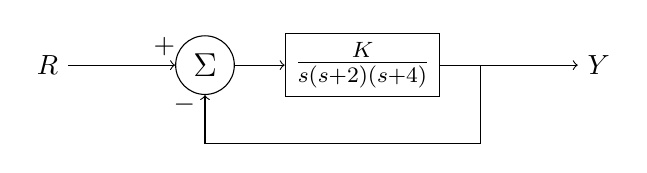
\begin{tikzpicture}[node distance = 2cm]
		\node[input] (r) at (0,0) {$ R $};
		\node[sum,right of=r] (sum) {\large$ \Sigma $};
		\node[block, right of=sum] (tf) {\large$ \frac{K}{s(s+2)(s+4)} $};
		\node[waypoint,below of=tf,node distance = 1cm] (wp) {};
		\node[output, right of=tf,node distance = 3cm] (y) {$ Y $};
		\draw[->] (r) -- node[above,pos=0.9] {$ + $} (sum);
		\draw[->] (sum) -- (tf);
		\draw[->] (tf) -- (y);
		\draw[->] ($(tf)!0.5!(y)$) |- (wp) -| node[left,pos=0.9] {$ - $} (sum);
		\end{tikzpicture}
	\end{center}
	Draw the real axis part of the root locus, and solve for $ \sigma $ and $ \theta $.
	\[ \sigma = \frac{0 + (-2) + (-4)}{3-0} = -2 \]
	\[ \theta = \frac{180^\circ + 360^\circ \ell}{3-0} =  60^\circ + 120^\circ \ell,\ \ell = 0,1,2 \quad\Rightarrow\quad \theta = 60^\circ,\ 180^\circ,\ 300^\circ \]
	\begin{center}
		\begin{tikzpicture}[scale=1]
		\draw (-6,0) -- (2,0);
		\draw (0,-2) -- (0,2);
		\node at (0,0) {\Large$ \times $};
		\draw[thick] (0,0.01) -- (-2,0.01);
		\node at (-2,0) {\Large$ \times $};
		\draw[thick] (-4,0.01) -- (-6,0.01);
		\node at (-4,0) {\Large$ \times $};
		\draw[thick] (-1,0) arc (180:150:3);
		\draw[thick] (-1,0) arc (180:210:3);
		\draw[dashed] (-0.845,-2) -- (-2,0) -- (-0.845,2);
		\end{tikzpicture}
	\end{center}
	What can we say about the stability of the closed-loop system?
	
	\nib If $ K $ is too large, the closed-loop system will be unstable.
	
	We will now graphically solve for the value of $ K $ that will make the system unstable. 
	\begin{center}
		\begin{tikzpicture}[scale=1] 
		\draw (-6,0) -- (2,0);
		\draw (0,-3.5) -- (0,3.5);
		\node at (0,0) {\Large$ \times $};
		\draw[thick] (0,0.01) -- (-2,0.01);
		\node at (-2,0) {\Large$ \times $};
		\draw[thick] (-4,0.01) -- (-6,0.01);
		\node at (-4,0) {\Large$ \times $};
		\draw[thick] (-1,0) arc (180:155:3);
		\draw[thick] (-1,0) arc (180:205:3);
		\draw[dashed] (0,-3.464) -- (-2,0) -- (0,3.464);
		\draw[thick] (-0.719,1.268) -- (0.322,3.5);
		\draw[thick] (-0.719,-1.268) -- (0.322,-3.5);
		\draw[dotted,->] (-4,0) -- node[above left] {$ M_{p1} $} (0,2.8) node {$ * $};
		\draw[dotted,->] (-2,0) -- node[above left,pos=0.25] {$ M_{p2} $} (0,2.8);
		\draw[dotted,->] (0,0) -- node[right] {$ M_{p3} $} (0,2.8);
		\end{tikzpicture}
	\end{center}
	We estimate the y-value where the locus crosses the imaginary axis (approximately $ s=2.8j $), and use the Pythagorean Theorem to find the magnitudes. From the Magnitude Criterion: $ K = M_{p1}M_{p2}M_{p3} $.
	\[ K \approx (4.88)(3.44)(2.80) = 47.0 \]
	
	We can verify our estimate by using the Routh-Hurwitz method:
	\[ \frac{Y}{R} = \frac{\frac{K}{s(s+2)(s+4)}}{1+\frac{K}{s(s+2)(s+4)}} = \frac{K}{s^3+6s^2+8s+K} \]
	\[ \begin{array}{c|c c}
	s^3 & 1 & 8\\
	s^2 & 6 & K\\
	s^1 & \frac{48-K}{6} & \\
	s^0 & K & \\
	\end{array} \]
	So, we have $ K>0 $ and $ K<48 $ as our requirements. Therefore, the locus in actuality crosses the imaginary axis at $ K=48 $. This is very close to our graphical estimate!\\
	
	Double check: A  third-order system with two poles on the imaginary axis has the form:
	\[ (s+ja)(s-ja)(s+b) = (s^2+a^2)(s+b) = s^3+bs^2+a^2s+a^2b \]
	At $ K=48 $:
	\[ s^3+6s^2+8s+48 \quad\Rightarrow\quad a=\sqrt{8},\ b = 6 \]
	Poles at: $ s=-6,\ \pm j2\sqrt{2} $.
	
	\section*{Break-Away and Break-In Points}
	The \textbf{Rule \#6} for root loci concerns break away and break in points. These are the points where the loci leaves or joins the real axis, respectively.
	\begin{itemize}
		\item[6.] The root locus leaves/enters the real axis at points that satisfy:
		\begin{equation}
		\sum^m \frac{1}{\sigma_b+z_i} = \sum^n \frac{1}{\sigma_b+p_i}
		\end{equation}
		where:
		\begin{itemize}
			\item $ \sigma_b $ is a break away/break in point
			\item $ n $ is the number of poles and $ m $ is the number of zeros
			\item the open loop zeros are: $ -z_1,-z_2,\ldots,-z_m $
			\item the open loop poles are: $ -p_1,-p_2,\ldots,-p_n $
		\end{itemize}
	\end{itemize}

We can derive this relationship by showing that the natural log of $ 1/L(\sigma_b) $ has a zero derivative at the same value of $ \sigma_b $ as $ 1/L(\sigma_b) $:

\begin{itemize}
	\item The closed-loop poles of the system can be found from:
	\[ 1+KL(s)=0 \]
	\item So, gain for the poles on the real axis ($ s=\sigma $) is given by
	\[ 1+KL(\sigma) = 0 \]
	\[ KL(\sigma) = -1 \]
	\[ K=\frac{-1}{L(\sigma)} \]
	\item Break-out points occur between two open-loop poles, where the $ K = 0 $ when the closed-loop poles are at the open-loop poles. Similarly, break-in points occur between two open-loop zeros (including the possibility of a zero at $ s=-\infty $), where $ K=\infty $ when the closed-loop poles are at the open-loop zeros. 
	\begin{center}
		\begin{tikzpicture}
		\begin{scope}[xshift = -7cm, yshift=1cm]
		\draw [<->] (0,2) node[left] {$ K $} |- (2,0) node[right] {$ \sigma $};
			\draw (1,0.25) parabola (0.25,2) (1,0.25) parabola (1.75,2);
		\end{scope}
		\begin{scope}[xshift = -3cm, yshift=1cm]
			\draw [<->] (0,2) node[left] {$ K $} |- (2,0) node[right] {$ \sigma $};
			\draw (1,1.75) parabola (0.25,0) (1,1.75) parabola (1.75,0);
		\end{scope}
		
		\draw[<->] (-8,0) -- (2,0) node[below left] {Re};
		\draw[<->] (0,-3) -- (0,3) node[below left] {Im};
		
		\node at (-1.25,0) {\large$ \times $};
		\node at (-2.75,0) {\large$ \times $};
		\node[below] at (-1.0625,-0.125) {\small$ K=0 $};
		\node[below] at (-2.9375,-0.125) {\small$ K=0 $};
		\draw[thick,-latex] (-1.25,0) -- (-2,0);
		\draw[thick,-latex] (-2.75,0) -- (-2,0);
		\draw[dotted] (-2,2.75) -- (-2,0) node[below] {$ \sigma_b $};
		\draw[fill=black] (-2,0) circle (0.05);
		
		\node at (-5.25,0) {\Large$ \circ $};
		\node at (-6.75,0) {\Large$ \circ $};
		\node[below] at (-5.0625,-0.125) {\small$ K=\infty $};
		\node[below] at (-6.9375,-0.125) {\small$ K=\infty $};
		\draw[thick,latex-latex] (-5.25,0) -- (-6.75,0);
		\draw[dotted] (-6,1.25) -- (-6,0) node[below] {$ \sigma_b $};
		\draw[fill=black] (-6,0) circle (0.05);
		\end{tikzpicture}
	\end{center}
	\item So, when looking along the real axis, we can say that $ K $ is at a maximum with respect to $ \sigma $ at break-out points, and at a minimum with respect to $ \sigma $ at break-in points. So, we can say that the break-in/break-out points occur at
	\[ \frac{dK(\sigma_b)}{d\sigma_b} = 0 \]
	\[ \frac{d}{d\sigma_b} \frac{-1}{L(\sigma_b)} = 0 \]
	\[ \Rightarrow \frac{d}{d\sigma_b} \frac{1}{L(\sigma_b)} = 0 \]
	This equation could be solved directly to find the values of $ \sigma_b $. In the following steps, we will show how Equation (12) above can be obtained from this.
	\item Consider the derivative of the natural log of $ 1/L(\sigma_b) $ when set equal to zero:
	\[ \frac{d}{d\sigma_b} \ln \left[ \frac{1}{L(\sigma_b)} \right] = L(\sigma_b) \frac{d}{d\sigma_b} \left[\frac{1}{L(\sigma_b)}\right] = 0 \]
	\item Since $ L(\sigma_b) $ is not zero at the breakaway or break-in points, letting
	\[ \frac{d}{d\sigma_b} \ln \left[ \frac{1}{L(\sigma_b)} \right] = 0 \]
	will thus yield the same value of $ \sigma_b $ as letting
	\[ \frac{d}{d\sigma_b} \left[ \frac{1}{L(\sigma_b)} \right] = 0 \]
	\item Hence,
	\begin{align*}
	\frac{d}{d\sigma_b} \ln \left[\frac{1}{L(\sigma_b)}\right] &= \frac{d}{d\sigma_b} \ln \left[ \frac{(\sigma_b+p_1)(\sigma_b+p_2)\cdots(\sigma_b+p_n)}{(\sigma_b+z_1)(\sigma_b+z_2)\cdots(\sigma_b+z_m)} \right] \\
	&= \frac{d}{d\sigma_b}\big[ \ln (\sigma_b+p_1) + \ln (\sigma_b+p_2) + \ldots + \ln (\sigma_b+p_n) \\ 
	& \quad - \ln (\sigma_b+z_1) - \ln (\sigma_b+z_2) - \ldots - \ln (\sigma_b+z_m) \big] \\
	& =\frac{1}{\sigma_b+p_1} + \frac{1}{\sigma_b+p_2} + \ldots + \frac{1}{\sigma_b+p_n} - \frac{1}{\sigma_b+z_1} - \frac{1}{\sigma_b+z_2} - \ldots - \frac{1}{\sigma_b+z_m}
	\end{align*}
	\item Thus,
	\[ \sum^m \frac{1}{\sigma_b+z_i} = \sum^n \frac{1}{\sigma_b+p_i} \]
	This equation can be solved for $ \sigma_b $, the real axis values that minimize or maximize $ K $, yielding the break-in or breakaway points.
\end{itemize}

Note that solving equation (12) may yield multiple values for $ \sigma_b $. You need to keep Rule 4 in mind to determine which of these solutions are feasible.

%	(6) is equivalent to solving $ \frac{d}{ds}L(s)\big|_{s=\sigma_b} = 0 $ for $ \sigma_b $.
%	
%	For example, consider 
%	\[ L(s) = \dfrac{(s+z)}{(s+p_1)(s+p_2)} \]
%	\[ \frac{d}{ds}L(s) = \dfrac{1}{(s+p_1)(s+p_2)} - \frac{(s+z)}{(s+p_1)^2(s+p_2)} - \frac{(s+z)}{(s+p_1)(s+p_2)^2} \]
%	\[ \frac{d}{ds}L(s) = \dfrac{(s+p_1)(s+p_2) - (s+z)(s+p_1) - (s+z)(s+p_2)}{(s+p_1)^2(s+p_2)^2} \]
%	\[ \frac{d}{ds}L(s)\big|_{s=\sigma_b} = \dfrac{(\sigma_b+p_1)(\sigma_b+p_2) - (\sigma_b+z)(\sigma_b+p_1) - (\sigma_b+z)(\sigma_b+p_2)}{(\sigma_b+p_1)^2(\sigma_b+p_2)^2} = 0 \]
%	\[ (\sigma_b+p_1)(\sigma_b+p_2) - (\sigma_b+z)(\sigma_b+p_1) - (\sigma_b+z)(\sigma_b+p_2) = 0 \]
%	\[ (\sigma_b+p_1)(\sigma_b+p_2) = (\sigma_b+z)\big( (\sigma_b+p_1) + (\sigma_b+p_2) \big) \]
%	\[ \dfrac{1}{\sigma_b+z} = \dfrac{(\sigma_b+p_1) + (\sigma_b+p_2)}{(\sigma_b+p_1)(\sigma_b+p_2)} \]
%	\[ \dfrac{1}{\sigma_b+z} = \dfrac{1}{\sigma_b+p_1} + \dfrac{1}{\sigma_b+p_2} \]
%	\[ \Updownarrow \]
%	\[ \sum^m \frac{1}{\sigma_b+z_i} = \sum^n \frac{1}{\sigma_b+p_i} \]
	
	
	
	\exmp
	Find the break away/break in points for the system shown.
	\begin{center}
		\begin{tikzpicture}[scale=0.75]
		\draw (-8,0) -- (2,0);
		\draw (0,-1.5) -- (0,1.5);
		\node at (0,0) {\Large$ \times $};
		\node[below right] at (-0,-0.1) {$ 0 $};
		\node at (-3,0) {\Large$ \times $};
		\node[below] at (-3,-0.1) {$ -3 $};
		\node at (-6,0) {\Large$ \circ $};
		\node[below] at (-6,-0.1) {$ -6 $};
		\end{tikzpicture}
	\end{center}
	\[ \frac{1}{\sigma_b+6} = \frac{1}{\sigma_b+3} + \frac{1}{\sigma_b+0} \]
	\[ \frac{1}{\sigma_b+6} = \frac{\sigma_b+(\sigma_b+3)}{\sigma_b (\sigma_b+3)}\]
	\[ \sigma_b(\sigma_b+3) = \sigma_b(\sigma_b+6)+(\sigma_b+6)(\sigma_b+3)\]
	\[ 0 = \sigma_b^2+12\sigma_b+18 \]
	\[ \sigma_b = -1.76,\ -10.25 \]
	\begin{center}
		\begin{tikzpicture}[scale=0.75]
		\draw (-12,0) -- (2,0);
		\draw (0,-3) -- (0,3);
		\node at (0,0) {\Large$ \times $};
		\node[below right] at (-0,-0.1) {$ 0 $};
		\node at (-3,0) {\Large$ \times $};
		\node[below] at (-3,-0.1) {$ -3 $};
		\node at (-6,0) {\Large$ \circ $};
		\node[below] at (-6,-0.1) {$ -6 $};
		\draw[thick] (-6,0) ellipse (4.25 and 4.25);
		\draw[thick,latex-latex] (-12,0)--(-6,0);
		\draw[thick] (-3,0) -- (0,0);
		\draw[-latex] (-3,0) -- (-2,0);
		\draw[-latex] (0,0) -- (-1.5,0);
		\node[below left] at (-10.25,-.0) {$ -10.25 $};
		\node[below right] at (-1.76,-.0) {$ -1.76 $};
		\draw[fill=black] (-10.25,-.0) circle (0.1);
		\draw[fill=black] (-1.76,-.0) circle (0.1);
		\end{tikzpicture}
	\end{center}
	\clearpage
	\section*{Angle of Departure/Arrival}
	Consider the following root locus. How can we determine the angle at which the locus leaves the complex poles?
	\begin{center}
		\begin{tikzpicture}[xscale=1.25]
		\draw (-4,0) -- (2,0);
		\draw (0,-3) -- (0,3);
		
		\node at (0,0) {\Large$ \times $};
		\node at (-2,2) {\Large$ \times $};
		\node at (-2,-2) {\Large$ \times $};
		
		\draw[dashed] (0.4,3) -- (-1.333,0) -- (0.4,-3);
		
		\draw[thick,-latex] (-2,2) node [above left] {$ s=-2+2j $} ..controls(-1.333,1) .. (0.2,3);
		\draw[thick,-latex] (-2,-2) node [below left] {$ s= -2-2j $} ..controls(-1.333,-1) .. (0.2,-3);
		
		\draw[thick,-latex] (0,0) node[below right] {$ s=0 $} -- (-4,0);
		
		\draw[dotted] (-2,2) -- (-1,2);
		\draw[dotted] (-2,-2) -- (-1,-2);
		\draw (-1.375,2) node[above] {$ \beta $} arc (0:-55:0.625);
		\draw (-1.375,-2) node[below] {$ \beta $} arc (0:55:0.625);
		
		\node[right] at (2.5,1) {\large$ \sigma = \frac{0+(-2+j2)+(-2-2j)}{3-0} = \frac{-4}{3} $};
		\node[right] at (2.5,0) {\large$ \theta = \frac{180^\circ\pm 360^\circ \ell}{3-0} = (2\ell+1) (60^\circ),\ \ell=0,\ 1,\ 2$};
		\node[right] at (2.5,-0.75) {\large$\quad= 60^\circ,\ 180^\circ,\ 300^\circ$};
		\end{tikzpicture}
	\end{center}
	The final root locus rule (\textbf{Rule \#7}) concerns the angle at which the locus departs an O.L. pole or arrives at an O.L. zero.
	\begin{itemize}
		\item[7.] The angle of departure/arrival of a complex pole/zero is given by:
		\[ \textrm{Pole Departure Angle:}\ \beta_p = \sum^m \theta_{zi} - \sum^{n-1} \theta_{pi} + 180 \pm\ell360 \]
		\[ \textrm{Zero Arrival Angle:}\ \beta_z = \sum^n \theta_{pi} - \sum^{m-1} \theta_{zi} + 180 \pm\ell360 \]
		where the $ \theta_{pi} $'s and $ \theta_{zi} $'s are the angles from all the other poles/zeros to the one in question. This relationship is derived from the Angle Criterion, $ \sum^m \theta_{zi} - \sum^{n} \theta_{pi} = -180 \pm\ell360 $
	\end{itemize}
	\exmp
	Find the angle of departure for the $ p_3 $ pole shown below.
	\begin{center}
		\begin{tikzpicture}[scale=0.75]
		\draw (-8,0) -- (4,0);
		\draw (0.5,-4) -- (0.5,4);
		\node at (2,0) {\Large$ \times $};
		\node at (-1,-3) {\Large$ \times $};
		\node at (-1,3) {\Large$ \times $};
		\node at (-7,0) {\Large$ \circ $};
		\node at (-4,0) {\Large$ \circ $};
		\draw[dashed] (2,0) -- (-1,3) -- (-1,-3);
		\draw[dashed] (-7,0) -- (-1,3) -- (-4,0);
		\draw (-6.25,0) arc (0:30:0.75);
		\draw (-3.25,0) arc (0:45:0.75);
		\draw (2.75,0) arc (0:135:0.75);	
		\draw (-0.25,-3) arc (0:90:0.75);
		\draw[dotted] (-1,-3) -- (0,-3);
		\node[above right] at (-6.25,0) {$ \theta_{z1} $};
		\node[above right] at (-3.25,0) {$ \theta_{z2} $};
		\node[above right] at (2.75,0) {$ \theta_{p2} $};
		\node[above right] at (-0.25,-3) {$ \theta_{p1} $};
		\end{tikzpicture}
	\end{center}
	\[ \beta_p = \theta_{z1}+\theta_{z2}-\theta_{p1}-\theta_{p2} + 180 \pm\ell360 \]
	
	\exmp
	Find the angle of departure for the pole at $ -2+2j $ shown below.
	
	\begin{center}
		\begin{tikzpicture}[scale=0.75]
		\draw (-4,0) -- (2,0);
		\draw (0,-3) -- (0,3);
		\node at (0,0) {\Large$ \times $};
		\node at (-2,-2) {\Large$ \times $};
		\node at (-2,2) {\Large$ \times $};
		\draw[dashed] (0,0) -- (-2,2) -- (-2,-2);
		\draw (0.75,0) arc (0:135:0.75);	
		\draw (-1.25,-2) arc (0:90:0.75);
		\draw[dotted] (-2,-2) -- (-1,-2);
		\node[above right] at (0.75,0) {$ \theta_{p2} $};
		\node[above right] at (-1.25,-2) {$ \theta_{p1} $};
		\end{tikzpicture}
	\end{center}
	\[ \beta_p = -\theta_{p1}-\theta_{p2} + 180 \pm\ell360 = -90-135+180\pm\ell360 \]
	\[ \beta_p = -45\pm\ell360 \]
	
	\section*{Plotting the root locus in Matlab}
	\begin{center}
		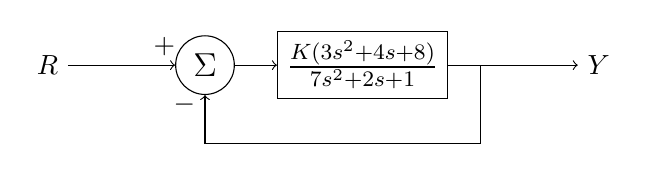
\begin{tikzpicture}[node distance = 2cm]
		\node[input] (r) at (0,0) {$ R $};
		\node[sum,right of=r] (sum) {\large$ \Sigma $};
		\node[block, right of=sum] (tf) {\large$ \frac{K(3s^2+4s+8)}{7s^2+2s+1} $};
		\node[waypoint,below of=tf,node distance = 1cm] (wp) {};
		\node[output, right of=tf,node distance = 3cm] (y) {$ Y $};
		\draw[->] (r) -- node[above,pos=0.9] {$ + $} (sum);
		\draw[->] (sum) -- (tf);
		\draw[->] (tf) -- (y);
		\draw[->] ($(tf)!0.5!(y)$) |- (wp) -| node[left,pos=0.9] {$ - $} (sum);
		\end{tikzpicture}
	\end{center}
	\paragraph{Step 1:} Define the open-loop transfer function (without $ K $).
	\begin{align*}
	&\texttt{>> G = tf(}\underbrace{\texttt{[3,4,8]}}_{\textrm{coef. of num.}}\texttt{,}\underbrace{\texttt{[7,2,1]}}_{\textrm{coef. of den.}}\texttt{)}\\
	\textrm{or} & \\
	& \texttt{>> s = tf('s');}\\
	& \texttt{>> G = (3*s\^{}2+4*s+8)/(7*s\^{}2+2*s+1)}\\
	\end{align*}
	\paragraph{Step 2:} Call the root locus command, \texttt{rlocus}
	\[ \texttt{>> rlocus(G)} \]
	
	\section*{Summary of Root Locus Rules}
	\begin{enumerate}
		\item Closed-loop poles start ($ K=0 $) at open-loop poles and end ($ K=\infty $) at open-loop zeros or infinity.
		\item There is one branch per open-loop pole.
		\item The locus is symmetric about the real axis.
		\item The real axis part of the root-locus lies to the left of an odd number of poles and zeros.
		\item Branches that go to infinity follow asymptotes that:
		\begin{itemize}
			\item Intersect the real axis at $ \sigma = \frac{\sum poles - \sum zeros}{n-m} $
			\item Have angle with the real axis $\theta = \frac{180^\circ\pm 360^\circ \ell}{n-m},\quad \ell = 0,\ 1,\ 2,\ \ldots $
			\item where $ n $ is the number of poles and $ m $ is the number of zeros.
		\end{itemize}
		\item Branches leave/enter the real axis at points $ \sigma_b $ that satisfy $ \sum^m \frac{1}{\sigma_b+z_i} = \sum^n \frac{1}{\sigma_b+p_i} $.
		\item The angle of departure/arrival of a complex zero/pole is given by
		\[ \textrm{Pole:}\ \beta = \sum^m \theta_{zi} - \sum^{n-1} \theta_{pi} + 180 \pm\ell360 \]
		\[ \textrm{Zero:}\ \beta = \sum^n \theta_{pi} - \sum^{m-1} \theta_{zi} + 180 \pm\ell360 \]
	\end{enumerate}
	
\end{document}
